% latex foo.tex 
% dvips -Poutline -G0 foo.dvi -o 
% ps2pdf -dPDFSETTINGS#/prepress foo.ps
\documentclass[slidestop,xcolor=pst,dvips]{beamer}
\usepackage{etex}
\usepackage{fancyvrb}
\usepackage{pstricks,pst-tree,pst-node,pst-plot,pst-3dplot}



\newcommand{\bi}{\begin{enumerate}}
\newcommand{\ei}{\end{enumerate}}
\newcommand{\sect}[1]{
\section{#1}
\begin{frame}[fragile]\frametitle{#1}
}

\newcommand{\grph}[2]{
\begin{columns}
\column{0.01\textwidth}
\column{0.6\textwidth}
\begin{pspicture}[showgrid=#1](-2,-2)(5,5)
#2
\end{pspicture}
}


\newcommand{\txt}[1]{
\column{0.4\textwidth}
\rput[bl](0,0){\parbox{\textwidth}{
\small
\begin{itemize}
#1
\end{itemize}}}
\end{columns}}

\newcommand{\myvec}[1]{
\pstThreeDDot[showpoints=true,drawCoor=true](#1)
\pstThreeDLine[arrows=->,linecolor=blue](0,0,0)(#1)
}


\mode<presentation>
{
%  \usetheme{Madrid}
  % or ...

%  \setbeamercovered{transparent}
  % or whatever (possibly just delete it)
}

\usepackage[english]{babel}

\usepackage[latin1]{inputenc}

\title[Transforms]
{
Transforms
}

\subtitle{} % (optional)

\author[Geoffrey Matthews]
{Geoffrey Matthews}
% - Use the \inst{?} command only if the authors have different
%   affiliation.

\institute[WWU/CS]
{
  Department of Computer Science\\
  Western Washington University
}
% - Use the \inst command only if there are several affiliations.
% - Keep it simple, no one is interested in your street address.

\date{Fall 2011}

% If you have a file called "university-logo-filename.xxx", where xxx
% is a graphic format that can be processed by latex or pdflatex,
% resp., then you can add a logo as follows:

%\pgfdeclareimage[height=0.5cm]{university-logo}{WWULogoProColor}
%\logo{\pgfuseimage{university-logo}}

% If you wish to uncover everything in a step-wise fashion, uncomment
% the following command: 

%\beamerdefaultoverlayspecification{<+->}

\begin{document}

\psset{arrowscale=2}

\begin{frame}
  \titlepage
\end{frame}

\newcommand{\myref}[1]{\small\item\url{#1}}
\newcommand{\myreff}[1]{\scriptsize\item\url{#1}}

%\begin{frame}
%  \frametitle{Outline}
%  \tableofcontents
%  % You might wish to add the option [pausesections]
%\end{frame}

\newcommand{\myframe}[4]{
\pstThreeDLine[arrows=->](#1)(#2)
\pstThreeDLine[arrows=->](#1)(#3)
\pstThreeDLine[arrows=->](#1)(#4)
}

\newcommand{\vtwo}[2]{
\left[\begin{array}{c} #1 \\ #2\end{array}\right]
}
\newcommand{\mtwo}[4]{
\left[\begin{array}{cc} #1 & #2 \\ #3 & #4\end{array}\right]
}
\newcommand{\vthree}[3]{
\left[\begin{array}{c} #1 \\ #2 \\ #3\end{array}\right]
}
\newcommand{\mthree}[9]{
\left[\begin{array}{ccc} #1&#2&#3\\#4&#5&#6\\#7&#8&#9\end{array}\right]
}
\newcommand{\vhomo}[1]{
\left[\begin{array}{c} #1 \\ 0\end{array}\right]
}
\newcommand{\phomo}[1]{
\left[\begin{array}{c} #1 \\ 1\end{array}\right]
}
\newcommand{\whomo}[1]{
\left[\begin{array}{c} #1 \end{array}\right]
}

\newcommand{\mhomo}[3]{
\left[\begin{array}{cccc} #1 \\ #2 \\ #3 \\0&0&0&1\end{array}\right]
}
\newcommand{\wmhomo}[4]{
\left[\begin{array}{cccc} #1 \\ #2 \\ #3 \\ #4\end{array}\right]
}

\sect{Transforms}
\grph{false}{
\psset{Alpha=60}
\pstThreeDCoor
\myframe{0,0,0}{1,0,0}{0,1,0}{0,0,1}
\myframe{-1,3,2}{-.01,3.3,1.8}{-1.25,3.9,2.33}{-0.67,2.75,2.9}
}
\txt{
\item Moving from one frame to another.
\item Describe an object in its own frame, then describe all points in the
  object in the world frame.
\item Describe the world in its natural frame, then describe
  everything in the world from the camera's frame.
\item Describe everything in the 3D world, then move it to the 2D
  world of the screen.
}
\end{frame}

\sect{Simple transformations}
\grph{false}{
\rput(-1,3){\pspolygon(0,0)(1,0)(1,2)}
\rput(-.5,3.25){\pspolygon[linecolor=blue](0,0)(1,0)(1,2)}
\rput(1,1){\pspolygon(0,0)(1,0)(1,2)}
\rput{30}(1,1){\pspolygon[linecolor=blue](0,0)(1,0)(1,2)}
\rput(3,-1){\pspolygon(0,0)(1,0)(1,2)}
\rput(3.5,-1){\pspolygon[linecolor=blue](0,0)(1.5,0)(1.5,3)}
}
\txt{
\item Translation
\item Rotation
\item Uniform scaling
}
\end{frame}

\sect{Transformations are used}
\begin{itemize}
\item Position objects in a scene
\item Change shape of objects
\item Create multiple copies of objects
\item Position camera
\item Projection for virtual cameras
\item Animations
\end{itemize}
\end{frame}

\sect{Rigid-body (Euclidean) Transforms}

\begin{pspicture}[showgrid=false](0,0)(10,6.5)
\psellipse(3,3)(2,.75)
\rput[b](2.75,3.75){\em \blue Rigid}
\rput(2,3){\small Translation}
\rput(3.75,3){\small Rotation}

\rput(8,4){\pspolygon(0,0)(1,0)(1,2)}
\rput{-30}(9.5,4){\pspolygon[linecolor=blue](0,0)(1,0)(1,2)}
\end{pspicture}
\begin{itemize}
\item Preserves distances and angles
\end{itemize}
\end{frame}

\sect{Similitudes / Similarity Transforms}

\begin{pspicture}[showgrid=false](0,0)(10,6.5)
\psellipse(4,3)(3.25,1.5)
\psellipse(3,3)(2,.75)
\rput[b](3.5,4.5){\em \blue Similarities}
\rput[b](2.75,3.75){\em \blue Rigid}

\rput(2,3){\small Translation}
\rput(3.75,3){\small Rotation}
\rput(6,3){\small Unif.~Scale}

\rput(8,4){\pspolygon(0,0)(1,0)(1,2)}
\rput(8.5,4){\pspolygon[linecolor=blue](0,0)(0.5,0)(0.5,1)}
\end{pspicture}
\begin{itemize}
\item Preserves angles
\end{itemize}
\end{frame}

\sect{Linear transforms}

\begin{pspicture}[showgrid=false](0,0)(10,6.5)
\psellipse(4,3)(3.25,1.5)
\psellipse(6,3)(3,1.5)
\psellipse(3,3)(2,.75)
\rput[b](3.5,4.5){\em \blue Similarities}
\rput[b](6.5,4.5){\em \blue Linear}
\rput[b](2.75,3.75){\em \blue Rigid}

\rput(2,3){\small Translation}
\rput(3.75,3){\small Rotation}
\rput(6,3){\small Unif.~Scale}
\rput(8.25,3){\small \parbox{1.5cm}{Scale\\Reflect\\Shear}}

\rput(10.5,2.5){\pspolygon(0,0)(1,0)(1,2)}
\rput(10.5,2.5){\pspolygon[linecolor=blue](0,0)(0.5,0)(0.5,3)}
\rput(10.5,2.5){\pspolygon[linecolor=blue](0,0)(-1,0)(-1,2)}
\rput(10.5,2.5){\pspolygon[linecolor=blue](0,0)(1,0)(1.5,2)}
\end{pspicture}
\begin{itemize}
\item $L(p+q) = L(p)+L(q)$
\item $L(ap) = aL(p)$
\end{itemize}

\end{frame}

\sect{Affine Transforms}

\begin{pspicture}[showgrid=false](0,0)(10,6.5)

\psellipse(5,3)(4.75,2.25)
\psellipse(4,3)(3.25,1.5)
\psellipse(6,3)(3,1.5)
\psellipse(3,3)(2,.75)

\rput[b](5,5.25){\em \blue Affine}
\rput[b](3.5,4.5){\em \blue Similarities}
\rput[b](6.5,4.5){\em \blue Linear}
\rput[b](2.75,3.75){\em \blue Rigid}

\rput(2,3){\small Translation}
\rput(3.75,3){\small Rotation}
\rput(6,3){\small Unif.~Scale}
\rput(8.25,3){\small \parbox{1.5cm}{Scale\\Reflect\\Shear}}

\rput(10.5,2.5){\pspolygon(0,0)(1,0)(1,2)}
\rput(10.5,2.5){\pspolygon(0,0)(1,0)(1,2)(0,2)}
\rput{-30}(8,0){\pspolygon[linecolor=blue](0,0)(1.5,0)(3,3)}
\rput{-30}(8,0){\pspolygon[linecolor=blue](0,0)(1.5,0)(3,3)(1.5,3)}
\end{pspicture}
\begin{itemize}
\item Preserves parallel lines
\end{itemize}
\end{frame}

\sect{Projective Transforms}

\begin{pspicture}[showgrid=false](0,0)(10,6.5)
\psellipse(5,3)(5,3)
\psellipse(5,3)(4.75,2.25)
\psellipse(4,3)(3.25,1.5)
\psellipse(6,3)(3,1.5)
\psellipse(3,3)(2,.75)
\rput[b](5,6){\em \blue Projective}
\rput[b](5,5.25){\em \blue Affine}
\rput[b](3.5,4.5){\em \blue Similarities}
\rput[b](6.5,4.5){\em \blue Linear}
\rput[b](2.75,3.75){\em \blue Rigid}

\rput(2,3){\small Translation}
\rput(3.75,3){\small Rotation}
\rput(6,3){\small Unif.~Scale}
\rput(8.25,3){\small \parbox{1.5cm}{Scale\\Reflect\\Shear}}
\rput(5,0.33){\small Perspective}

\rput(10,4){
\psline(0,0)(2,0)
\psline(0,1)(2,1)
\psline(0,2)(2,2)
\psline(0,0)(0,2)
\psline(1,0)(1,2)
\psline(2,0)(2,2)
}
\rput(10,1){
\psset{linecolor=blue}
\psline(0.3,0.5)(2,0)
\psline(0.3,1)(2,1)
\psline(0.3,1.5)(2,2)
\psline(0.3,0.5)(0.3,1.5)
\psline(1.1,0.25)(1.1,1.75)
\psline(2,0)(2,2)
}
\end{pspicture}
\begin{itemize}
\item Preserves lines
\end{itemize}

\end{frame}

\sect{Homogeneous coordinates}
\begin{itemize}
\item Recall a 3D frame is three vectors and a point: ${x,y,z,p}$.
\item We can represent a point $q$ as {\em coordinates} in this frame
as a 4-vector $(a,b,c,1)$ because $q= [x,y,z,p]\cdot [a,b,c,1]^T$
\item Likewise we can represent a vector $v$ as {\em coordinates} in
this frame with a 4-vector $(a,b,c,0)$ because $v =
[x,y,z,p]\cdot[a,b,c,0]^T$ 
\item These are called {\em homogeneous coordinates}
\item They help distinguish between points and vectors
\item They simplify other calculations with points and vectors,
in particular, transformations.
\end{itemize}
\end{frame}

\sect{Representing transforms with matrices}
\begin{itemize}
\item A general linear transformation:
\begin{eqnarray*}
x' &=& ax + by + c\\
y' &=& dx + ey + f
\end{eqnarray*}
\item Multiplication and addition:
\begin{eqnarray*}
\vtwo{x'}{y'} &=& \mtwo{a}{b}{d}{e} \vtwo{x}{y} + \vtwo{c}{f}\\
p' &=& Mp + t
\end{eqnarray*}
\end{itemize}
\end{frame}

\sect{Homogeneous coordinates}
\begin{itemize}
\item If we add another dimension, we can get by with just multiplication.
\begin{eqnarray*}
x' &=& ax + by + c\\
y' &=& dx + ey + f\\
1 &=& 1\\
\vthree{x'}{y'}{1} &=& \mthree abcdef001 \vthree xy1\\
p' &=& Mp
\end{eqnarray*}
\item In 2D we use $3\times 3$ matrices.
\end{itemize}
\end{frame}

\sect{Homogeneous coordinates}
\begin{itemize}
\item In 3D we use $4\times 4$ matrices.
\item Each point has an extra value, $w$, usually 1.
\begin{eqnarray*}
x' &=& ax+by+cz+d\\
y' &=& ex+fy+gz+h\\
z' &=& ix+jy+kz+l\\
\phomo{x'\\y'\\z'} &=& 
\mhomo{a&b&c&d}{e&f&g&h}{i&j&k&l} \phomo{x\\y\\z}\\
p' &=& Mp
\end{eqnarray*}
\end{itemize}
\end{frame}

\sect{Homogeneous coordinates}
\begin{itemize}
\item Each point has an extra value, $w$, usually 1.
\item If $M$ is an {\em affine} transformation, $w$ will remain 1.
\item We use $w\not=1$ only in projections.
\item If $w\not=1$ for a point, we normalize by dividing by $w$ before using.
\begin{eqnarray*}
\wmhomo{a&b&c&d}{e&f&g&h}{i&j&k&l}{m&n&o&p} \whomo{x\\y\\z\\1}&=& 
\whomo{x'\\y'\\z'\\w'} \\
&\Leftrightarrow&\whomo{x'/w'\\y'/w'\\z'/w'\\1} \\
Mp &=& p'
\end{eqnarray*}
\end{itemize}
\end{frame}

\newcommand{\mvpoint}[2]{
\psline[showpoints=true,linestyle=none](#1)(#2)
\psline[arrows=->,linecolor=blue](#1)(#2)
}

\sect{Translate}
\begin{pspicture}[showgrid=false](0,0)(2,2)
\psline[arrows=<->](2,0)(0,0)(0,2)
\mvpoint{1,1}{2,1.5}
\mvpoint{1,0.5}{2,1}
\mvpoint{.5,1.5}{1.5,2}
\end{pspicture}
\begin{eqnarray*}
\phomo{x'\\y'\\z'} &=& \mhomo{1&0&0&t_x}{0&1&0&t_y}{0&0&1&t_z}\phomo{x\\y\\z}
\end{eqnarray*}

\end{frame}

\sect{Scale}
\begin{pspicture}[showgrid=false](0,0)(2,2)
\psline[arrows=<->](2,0)(0,0)(0,2)
\mvpoint{1,1}{2,2}
\mvpoint{1,0.25}{2,.5}
\mvpoint{.25,1}{.5,2}
\end{pspicture}
\begin{eqnarray*}
\phomo{x'\\y'\\z'} &=& \mhomo{s_x&0&0&0}{0&s_y&0&0}{0&0&s_z&0}\phomo{x\\y\\z}
\end{eqnarray*}
\begin{itemize}
\item Isotropic (uniform) scaling: $s_x=s_y=s_z$.
\item Generally avoid scaling;  creates difficulties with normals.
\end{itemize}
\end{frame}

\sect{Rotation}
\begin{pspicture}[showgrid=false](-1,-1)(2,2)
\psline[arrows=<->](2,0)(0,0)(0,2)
\psline[arrows=->](0,0)(-0.5,-1)
\rput(2,-.2){$x$}
\rput(-.2,2){$y$}
\rput(-1,-1){$z$}
\psline[showpoints=true,linestyle=none](1.5,.5)(.5,1.5)
\psline[linestyle=dashed](1.5,.5)(0,0)(.5,1.5)
\psarc[arrows=->,linecolor=blue](0,0){1.6}{20}{70}
\rput(.5,.5){$\theta$}
\end{pspicture}
\begin{itemize}
\item Righthand rotation about the $z$ axis in a righthand frame.
\item Lefthand rotation about the $z$ axis in a lefthand frame.
\begin{eqnarray*}
\phomo{x'\\y'\\z'} &=& \mhomo{\cos(\theta)&-\sin(\theta)&0&0}{\sin(\theta)&\cos(\theta)&0&0}{0&0&1&0}\phomo{x\\y\\z}
\end{eqnarray*}
\end{itemize}
\end{frame}

\sect{Rotation}
\begin{itemize}
\item Righthand rotation about the $x$ axis.
\begin{eqnarray*}
\phomo{x'\\y'\\z'} &=& 
\mhomo{1&0&0&0}
      {0&\cos(\theta)&-\sin(\theta)&0}
      {0&\sin(\theta)&\cos(\theta)&0}\phomo{x\\y\\z}
\end{eqnarray*}
\item Righthand rotation about the $y$ axis.
\begin{eqnarray*}
\phomo{x'\\y'\\z'} &=& 
\mhomo{\cos(\theta)&0&-\sin(\theta)&0}
      {0&1&0&0}
      {\sin(\theta)&0&\cos(\theta)&0}\phomo{x\\y\\z}
\end{eqnarray*}
\item Righthand rotation about the $z$ axis.
\begin{eqnarray*}
\phomo{x'\\y'\\z'} &=& 
\mhomo{\cos(\theta)&-\sin(\theta)&0&0}
      {\sin(\theta)&\cos(\theta)&0&0}
      {0&0&1&0}\phomo{x\\y\\z}
\end{eqnarray*}
\end{itemize}
\end{frame}

\sect{Rotation about an arbitrary axis}

\begin{itemize}
\item
Rodrigues rotation matrix

\url{http://en.wikipedia.org/wiki/Rotation_matrix}

\item Fairly easy derivation using vectors.
\item Can also use quaternions.
\item
We will find other ways to deal with arbitrary rotations.
\end{itemize}

\end{frame}

\newcommand{\bluebox}[4]{
\pspolygon[showpoints=true,fillstyle=solid,fillcolor=blue](#1,#2)(#1,#4)(#3,#4)(#3,#2)
\rput[tr](#1,#2){\tiny$(#1,#2)$}
\rput[bl](#3,#4){\tiny$(#3,#4)$}
}


\sect{How are tranforms combined?}
\psset{unit=0.2cm}
\begin{pspicture}(-1,0)(8,5)
\psline[arrows=<->](8,0)(0,0)(0,5)
\bluebox 0011
\end{pspicture}
{\small Scale(2,2) $\Rightarrow$}
\begin{pspicture}(-1,0)(8,5)
\psline[arrows=<->](8,0)(0,0)(0,5)
\bluebox 0022
\end{pspicture}
{\small Translate(3,1) $\Rightarrow$}
\begin{pspicture}(-1,0)(8,5)
\psline[arrows=<->](8,0)(0,0)(0,5)
\bluebox 3153
\end{pspicture}

\bigskip

\begin{itemize}
\item Matrix multiplication is associative: $p' = T(Sp) = TS p$
\[
TS = \mthree 103011001 \mthree 200020001 = \mthree 203021001
\]
\item Remember we multiply on the left, so in matrix $TS$ scale is done first, translate second.
\end{itemize}

\psset{unit=1cm}
\end{frame}

\sect{Matrix multiplication is not commutative: $TS\not=ST$}
\psset{unit=0.2cm}
\begin{pspicture}(-1,0)(8,5)
\psline[arrows=<->](8,0)(0,0)(0,5)
\bluebox 0011
\end{pspicture}
{\small Scale(2,2) $\Rightarrow$}
\begin{pspicture}(-1,0)(8,5)
\psline[arrows=<->](8,0)(0,0)(0,5)
\bluebox 0022
\end{pspicture}
{\small Translate(3,1) $\Rightarrow$}
\begin{pspicture}(-1,0)(8,5)
\psline[arrows=<->](8,0)(0,0)(0,5)
\bluebox 3153
\end{pspicture}

\[
TS = \mthree 103011001 \mthree 200020001 = \mthree 203021001
\]

\begin{pspicture}(-1,0)(8,5)
\psline[arrows=<->](8,0)(0,0)(0,5)
\bluebox 0011
\end{pspicture}
{\small Translate(3,1) $\Rightarrow$}
\begin{pspicture}(-1,0)(8,5)
\psline[arrows=<->](8,0)(0,0)(0,5)
\bluebox 3142
\end{pspicture}
{\small Scale(2,2) $\Rightarrow$}
\begin{pspicture}(-1,0)(8,5)
\psline[arrows=<->](8,0)(0,0)(0,5)
\bluebox 6284
\end{pspicture}

\[
ST = \mthree 200020001 \mthree 103011001 = \mthree 206022001
\]

\psset{unit=1cm}

\end{frame}
\sect{Easy inverses}
\begin{itemize}
\item The inverse of a rotation matrix is its transpose.
\end{itemize}
\end{frame}
\sect{Easy inverses}
\begin{eqnarray*}
\mhomo{1 & 0 & 0 & x}
{0 & 1 & 0 & y}
{0 & 0 & 1 & z}^{-1} 
&=&\pause
\mhomo{1 & 0 & 0 & -x}
{0 & 1 & 0 & -y}
{0 & 0 & 1 & -z}
\\\pause
\mhomo{x & 0 & 0 & 0}
{0 & y & 0 & 0}
{0 & 0 & z & 0}^{-1}
&=&\pause
\mhomo{1/x & 0 & 0 & 0}
{0 & 1/y & 0 & 0}
{0 & 0 & 1/z & 0}
\\\pause
\mhomo{c & -s & 0 & 0}
{s & c & 0 & 0}
{0 & 0 & 1 & 0}^{-1} 
&=&\pause
\mhomo{c & s & 0 & 0}
{-s & c & 0 & 0}
{0 & 0 & 1 & 0}
\end{eqnarray*}

\end{frame}

\sect{Decomposable Transforms}
\begin{eqnarray*}
\mhomo{1 & 0 & 0 & x}
{0 & 1 & 0 & y}
{0 & 0 & 1 & z}
\mhomo{c & -s & 0 & 0}
{s & c & 0 & 0}
{0 & 0 & 1 & 0}
 &=&\pause
\mhomo{c & -s & 0 & x}
{s & c & 0 & y}
{0 & 0 & 1 & z}
\\\pause
\mhomo{c & -s & 0 & 0}
{s & c & 0 & 0}
{0 & 0 & 1 & 0}
\mhomo{1 & 0 & 0 & x}
{0 & 1 & 0 & y}
{0 & 0 & 1 & z} 
&=&\pause
\mhomo{c & -s & 0 & cx-sy}
{s & c & 0 & sx+cy}
{0 & 0 & 1 & z}
\end{eqnarray*}

\end{frame}


\sect{Decomposable Transforms}
\begin{eqnarray*}
\mhomo{1 & 0 & 0 & x}
{0 & 1 & 0 & y}
{0 & 0 & 1 & z}
\mhomo{a & 0 & 0 & 0}
{0 & b & 0 & 0}
{0 & 0 & c & 0}
 &=&\pause
\mhomo{a & 0 & 0 & x}
{0 & b & 0 & y}
{0 & 0 & c & z}
\\\pause
\mhomo{a & 0 & 0 & 0}
{0 & b & 0 & 0}
{0 & 0 & c & 0}
\mhomo{1 & 0 & 0 & x}
{0 & 1 & 0 & y}
{0 & 0 & 1 & z} 
&=&\pause
\mhomo{a & 0 & 0 & ax}
{0 & b & 0 & by}
{0 & 0 & c & cz}
\end{eqnarray*}

\end{frame}

\sect{More Easy Inverses}
\begin{eqnarray*}
\mhomo{c & -s & 0 & x}
{s & c & 0 & y}
{0 & 0 & 1 & z}^{-1}
&=& \pause
\left(\mhomo{1 & 0 & 0 & x}
{0 & 1 & 0 & y}
{0 & 0 & 1 & z}
\mhomo{c & -s & 0 & 0}
{s & c & 0 & 0}
{0 & 0 & 1 & 0}\right)^{-1}\\
&=& \pause
\mhomo{c & -s & 0 & 0}
{s & c & 0 & 0}
{0 & 0 & 1 & 0}^{-1}
\mhomo{1 & 0 & 0 & x}
{0 & 1 & 0 & y}
{0 & 0 & 1 & z}^{-1}\\
&=& \pause
\mhomo{c & s & 0 & 0}
{-s & c & 0 & 0}
{0 & 0 & 1 & 0}
\mhomo{1 & 0 & 0 & -x}
{0 & 1 & 0 & -y}
{0 & 0 & 1 & -z}
\end{eqnarray*}
\end{frame}

\sect{More Easy Inverses}
\begin{eqnarray*}
\mhomo{a & 0 & 0 & x}
{0 & b & 0 & y}
{0 & 0 & c & z}^{-1}
&=&\pause
\left(\mhomo{1 & 0 & 0 & x}
{0 & 1 & 0 & y}
{0 & 0 & 1 & z}
\mhomo{a & 0 & 0 & 0}
{0 & b & 0 & 0}
{0 & 0 & c & 0}\right)^{-1}\\
&=&\pause
\mhomo{a & 0 & 0 & 0}
{0 & b & 0 & 0}
{0 & 0 & c & 0}^{-1}
\mhomo{1 & 0 & 0 & x}
{0 & 1 & 0 & y}
{0 & 0 & 1 & z}^{-1}\\
&=&\pause
\mhomo{1/a & 0 & 0 & 0}
{0 & 1/b & 0 & 0}
{0 & 0 & 1/c & 0}
\mhomo{1 & 0 & 0 & -x}
{0 & 1 & 0 & -y}
{0 & 0 & 1 & -z}
\end{eqnarray*}
\end{frame}


\sect{The Modelview Matrix}
\begin{itemize}
\item Most worlds are modelled by
\begin{enumerate}
\item  positioning the model
in world coordinates
\item position the camera in world coordinates
\end{enumerate}
\item To put all objects in camera coordinates
\begin{enumerate}
\item multiply each object by model transform 
\item multiply by  inverse camera transform
\end{enumerate}

\item The product of these two matrices is called the {\bf modelview}
matrix:
\[
C^{-1}M
\]
\item Each point in an object will be multiplied by this matrix to put it
into camera coordinates.
\end{itemize}

\end{frame}

\sect{Finding a frame}
\begin{itemize}
\item When positioning a model or camera in the world it is generally
  easy to find a {\em forward} vector {$\bf v_1$}
 and an {\em up} {$\bf v_2$} vector in world
  coordinates. 
\item These two vectors need not be orthonormal, just not parallel.
\item A third vector, pointing {\em right}, can be defined as $\bf
v_3 =  v_1\times v_2$.
\item Using the
  \href{http://en.wikipedia.org/wiki/Gram-Schmidt_process}{\bf Gram Schmidt} 
process you can create an orthonormal frame $\bf e_1,e_2,e_3$ from
$\bf v_1, v_2, v_3$
\pause

\item Slightly faster to Gram-Schmidt-ize the {\em forward} and {\em
    up} vectors, then the cross product is automatically orthonormal.
\item It is usually easy to find a {\em forward} vector for an object---what
  is it ``looking at''?
\item An {\em up} vector is also usually easy, can almost always start with
  $(0,1,0)$ and then Gram-Schmidt it.
\item Use {\em forward}$\times${\em up} to get {\em right}.

\end{itemize}
\end{frame}

\sect{Change of frame}
\centerline{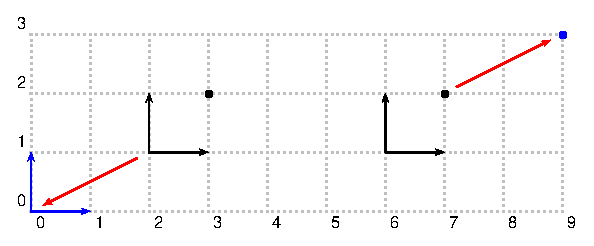
\includegraphics{figures/framevsobject.eps}}
\begin{itemize}
\item Does a transform move the object or the frame?\pause
\item Transform for the above:
\[
\left[\begin{array}{cccc}
1 & 0 & 0 & 2\\ 0 & 1 & 0 & 1\\ 0 & 0 & 1 & 0 \\ 0 & 0 & 0 & 1
\end{array}\right]
\]
\pause
\item Note that these are {\em not} inverses!  Just a different vocabulary.
\pause
\item However, if you want to {\em move a frame}, you need an inverse.
\end{itemize}
\end{frame}

\sect{Change of frame}
\begin{columns}
\column{0.5\textwidth}
{\small
\begin{eqnarray*}
\mhomo
{a & d & g & j }
{b & e & h & k}
{c & f & i & l}
\vhomo{1\\0\\0}
 &=& \vhomo{a\\b\\c}\\
\mhomo
{a & d & g & j }
{b & e & h & k}
{c & f & i & l}
\vhomo{0\\1\\0}
 &=& \vhomo{d\\e\\f}\\
\mhomo
{a & d & g & j }
{b & e & h & k}
{c & f & i & l}
\vhomo{0\\0\\1}
 &=& \vhomo{g\\h\\i}\\
\mhomo
{a & d & g & j }
{b & e & h & k}
{c & f & i & l}
\phomo{0\\0\\0}
 &=& \phomo{j\\k\\l}\\
\end{eqnarray*}
}
\pause
\column{0.5\textwidth}
\begin{eqnarray*}
(\vec{v_1}, \vec{v_2}, \vec{v_3}, \vec{p})\cdot\vec{x} &=& \vec{v_1}\\\\
(\vec{v_1}, \vec{v_2}, \vec{v_3}, \vec{p})\cdot\vec{y} &=& \vec{v_2}\\\\
(\vec{v_1}, \vec{v_2}, \vec{v_3}, \vec{p})\cdot\vec{z} &=& \vec{v_3}\\\\
(\vec{v_1}, \vec{v_2}, \vec{v_3}, \vec{p})\cdot\vec{o} &=& \vec{p}
\end{eqnarray*}
\end{columns}
\end{frame}


\sect{Change of Frame}
\grph{false}{
\psset{Alpha=60}
\pstThreeDCoor
\myframe{0,0,0}{1,0,0}{0,1,0}{0,0,1}
\myframe{-1,3,2}{-.01,3.3,1.8}{-1.25,3.9,2.33}{-0.67,2.75,2.9}
\pstThreeDPut(-1,3.2,1.8){$\vec{p}$}
\pstThreeDPut(-.01,3.3,1.6){$\vec{v_1}$}
\pstThreeDPut(-1.25,4.1,2.3){$\vec{v_2}$}
\pstThreeDPut(-0.67,2.7,3.2){$\vec{v_3}$}
}
\column{0.4\textwidth}
\rput[bl](0,0){\parbox{\textwidth}{
\begin{eqnarray*}
(\vec{v_1}, \vec{v_2}, \vec{v_3}, \vec{p})\cdot\vec{x} &=& \vec{v_1}\\\\
(\vec{v_1}, \vec{v_2}, \vec{v_3}, \vec{p})\cdot\vec{y} &=& \vec{v_2}\\\\
(\vec{v_1}, \vec{v_2}, \vec{v_3}, \vec{p})\cdot\vec{z} &=& \vec{v_3}\\\\
(\vec{v_1}, \vec{v_2}, \vec{v_3}, \vec{p})\cdot\vec{o} &=& \vec{p}
\end{eqnarray*}
\pause
\begin{itemize}
\item Use to put model points into the world.
\pause
\item Use inverse to put the world in camera coords.
\end{itemize}
}}
\end{columns}
\end{frame}


\sect{Camera transforms}
\grph{false}{
\psset{Alpha=60}
\pstThreeDCoor
\myframe{0,0,0}{1,0,0}{0,1,0}{0,0,1}
\myframe{-1,3,2}{-.01,3.3,1.8}{-1.25,3.9,2.33}{-0.67,2.75,2.9}
\pstThreeDPut(-1,3.2,1.8){$\vec{p}$}
\pstThreeDPut(-.01,3.3,1.6){$\vec{v_1}$}
\pstThreeDPut(-1.25,4.1,2.3){$\vec{v_2}$}
\pstThreeDPut(-0.67,2.7,3.2){$\vec{v_3}$}
}
\column{0.4\textwidth}
\rput[bl](0,0){\parbox{\textwidth}{
\begin{itemize}
\item Cameras and objects
generally use only rotation and translation.
\item Can use ``easy inverse'' for cameras.
\end{itemize}
}}
\end{columns}
\end{frame}

\sect{Transforming normals}
\centerline{
\includegraphics{figures/normaltransform.eps}}
\begin{itemize}
\item Normals do not stay normalized after scale transforms.
\item Must use the inverse transpose
\[
\left(M^{-1}\right)^T
\]
\item Might be good to maintain inverses.
\item Rigid transforms OK.
\end{itemize}
\end{frame}

\sect{Online Resources}
{\bf Readings}
\begin{itemize}
\myref{http://en.wikipedia.org/wiki/Transformation_matrix}
\myref{http://xkcd.com/184/}
\myreff{http://ocw.mit.edu/courses/electrical-engineering-and-computer-science/}, Computer graphics

\myref{http://www.songho.ca/opengl/index.html}
\end{itemize}

\vfill

\centerline{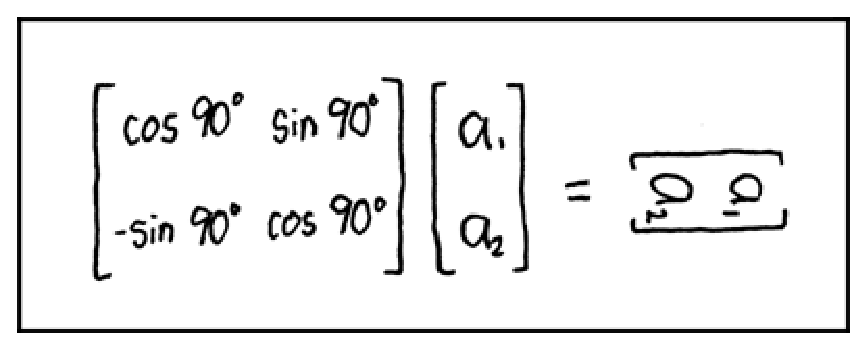
\includegraphics[scale=0.5]{figures/matrix_transform.eps}}

\end{frame}


\end{document}
